% Define block styles
\tikzstyle{block} = [draw, rectangle, text centered, text width=10em, minimum height=0.5em, rounded corners=true]
\tikzstyle{arrowtext} = [text width=4em, text centered]
\tikzstyle{arrow} = [draw, -latex]

\definecolor{red1}{RGB}{160,0,0}
\definecolor{green1}{RGB}{0,160,0}
\definecolor{blue1}{RGB}{0,0,160}

\usetikzlibrary{shapes.geometric,arrows,positioning}

	      
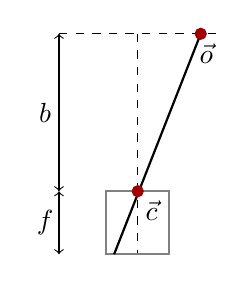
\begin{tikzpicture}[node distance=4em, auto]
    % Draw axis
    \draw [-, dashed] (0,0) |- (0,-2.8);
    \draw [-, dashed] (-1,0) |- (1,0);

    % camera
    %\draw [-, thick, gray] (-0.5,-2)
    %    -- (0.5,-2)
    %    -- (0.3,-2.3)
    %    -- (-0.3,-2.3)
    %    -- (-0.5,-2);
    \draw [-, thick, gray] (0.4,-2.0) 
        -- (0.4,-2.8)
        -- (-0.4,-2.8)
        -- (-0.4,-2.0)
        -- cycle;

    % light
    \draw[-, thick] (0.8,0) -- (-0.3,-2.8);

    % point
    \draw[fill=red1, color=red1] (0.8,0) circle (2pt) node [below, color=black, xshift=0.2em] {$\vec{o}$};
    \draw[fill=red1, color=red1] (0,-2.0) circle (2pt) node [below, color=black, xshift=0.5em] {$\vec{c}$};

    % sizes
    \path[<->]
        (-1.0,0) edge node [xshift=-0.5em, anchor=center] {$b$} (-1.0,-2.0)
        (-1.0,-2.0) edge node [xshift=-0.5em, anchor=center] {$f$} (-1.0,-2.8);
\end{tikzpicture}
